\section*{Method}
\label{Method}
%
The method of choice in this paper is Principal Component Analysis (PCA). This method is typically used as an explorative technique to obtain an overview by reducing a complex data set to a lower number of dimensions. The dimensions found in PCA is called principal components (PC). Each PC explains a certain amount variation noted in percentage which describes how much of the variances of the original variables, the PC describes.\blankline
%
PCA uses linear algebra to extract the components. The PCA consists of different steps, an overview of these different steps is listed based on \textcite[pp. 211-213]{Naes2010}:

\begin{enumerate}
	\item Organise the data in a data matrix where each row in the table corresponds to an ‘object’ and each column to a ‘variable’
	\item Computing the average of all the variables. 
	\item The averages are subtracted from their corresponding variables.
	\item Search for the direction in space that has as large variance as possible, which is the first principal component (PC1).
	\item Search for the second principal component(PC2). Same procedure as for PC1, but under the restriction that the direction of the PC2 is orthogonal to PC1. 
	\item Extract new components that describe as much variance as possible under the restriction that each new PC-direction is orthogonal to the previous.
	\item Stop extraction when the desired number of components have been extracted. In many cases 2-3 components is enough to explain most of the variation. 
\end{enumerate}
\blankline
%
The variances of each PC is noted in percentage.
The sum of the variances of the PC's is equal to the sum of the variances of the original variables. This means that if we have two components, the sum of this two components describes the total percentage covered be them. An example could be PC1 = 87 \% and PC2 = 9 \%. The total variances covered be having two components in this case will be 87 \% + 9 \% = 96 \% \parencite[p. 213]{Naes2010}. This could be useful when determine when the desired number of components has been extracted. To get an overview of the total variances covered be each number of dimensions a scree-plot can be made, which shows exactly this. \blankline
%
%Score value is the principal component value 
The results of the PCA is typically presented graphically in a scatter plot in two- or three-dimensions, where each dimension is based on a PC. There is different types of plots relevant to make when conducting PCA. 

\subsection*{Score plot}
The score plot gives an overview of the relation between the rating of the different object and there relation to PC for the plot. \blankline
%An example of a score plot in two dimensions is presented in \autoref{fig:PlotExample}. 
%
%\begin{figure}[H]
%\centering
%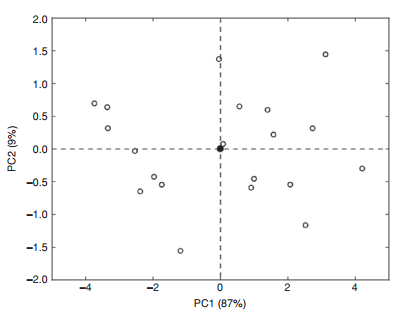
\includegraphics[width =0.7\textwidth]{Figure/PlotExample}
%\caption{Example of two-dimension score plot \parencite[p. 215]{Naes2010}.}
%\label{fig:PlotExample}
%\end{figure}
%\noindent
%
On a score plot the samples are plotted and if two samples are close to each other in the plot it means that they have similar overall properties and if the samples are fare away from each other in the plot it means that they are very different. It is important to take in to account the chosen number of dimensions. Some samples can be close to each other, and therefore similar, in two dimension but no longer close to each other if an extra dimension is added. 
%
\subsection*{Loading plot}
The other plot used when conducting PCA is loadings plot where the loading values are plotted.
Loading values defines the contribution of each of the original variables in the calculation of the first score. This means that a high loading value for a specific variable indicates that this variable is strongly related to the PC, that the loading value is according to \parencite[p. 212]{Naes2010}. \blankline
%
The loading plot is used to see which variables are correlated, by looking at which variables are plotted close to each other. If two variables are places on opposite sides of the origin(0,0) it means that these two variables are negative correlated \parencite[p. 216]{Naes2010}. 
%
\subsection*{Bi-plot}
If a score plot and a loading plot is plotted together in the same plot it is called a bi-plot  \parencite[p. 217]{Naes2010}. The advances of doing this is that it saves places in the paper. Other than that there isn't a big different between making a score plot and a loading plot or just making a bi-plot, it is primarily based on the preference of the author. The bi-plot is interpreted according to the score values in the same way as in the score plot and according to loading values in the same way as the loading plot is interpreted. 
%
\subsection*{Redundant}
Redundancy means that some attributes, measured in the data, is highly correlated. 
In some cases redundant attributes are both highly correlated and measuring the same thing, but this is not always the case. It is possible to have to very different attributes that aren't the same thing but still highly correlated. \blankline
%
If there is redundancy in a dataset, it often means that variance from a large number of attributes can be described with only a few number of principal components and in this way give an easy overview of the data. 